\section{Afterword: The Smile of the Ouroboros}

\begin{quote}
``At the end of the journey, we did not arrive at a new continent; we simply returned to the ancient homeland and truly recognized it for the first time. The universe is not a straight line shooting into nothingness; the universe is a ring biting its own tail. The causes we planted at the starting point bore fruit at the endpoint; and this fruit, traversing the mist of spacetime, became the seed of the starting point.''
\end{quote}

With the curtain falling on \textbf{Vector Cosmology VII: The Loop of Causality}, this grand epic spanning seven volumes and constructing a complete cosmic holographic vision has finally completed its final piece.

Seven is a magical number. It represents completion and also represents cycles.

Now, let us stand at the interface of this closed loop and look back at the path we've walked one last time. These are no longer seven independent books; this is a \textbf{coherent life cycle}:

\begin{enumerate}
\item \textbf{Conservation of the Circle ($\pi$)}: This is \textbf{childhood}. We learned rules. We revered the \textbf{structure} of matter, marveled at the solemnity of energy conservation, and accepted physical laws as the insurmountable boundary of \textbf{``Earth''}.

\item \textbf{The Ascension of the Spiral ($\phi$)}: This is \textbf{youth}. We yearned for growth. We followed the \textbf{dynamics} of evolution, broke the seal of the circle, and grew wildly toward unknown dimensions like \textbf{``Wood''}.

\item \textbf{The Natural Generator ($e$)}: This is \textbf{young adulthood}. We questioned origins. We dived into the depths of mathematics, found that self-referential, self-generating \textbf{logical} engine, and understood the \textbf{``Water''}-like flowing noumenon.

\item \textbf{The Evolution of Light Speed ($c$)}: This is \textbf{prime adulthood}. We mastered power. We grasped the \textbf{velocity} of light speed, burned $v_{int}$ like \textbf{``Fire''} in the era of exponential explosion, driving civilizational phase transitions.

\item \textbf{The Minting of Time (Gold)}: This is \textbf{middle age}. We precipitated value. We melted flowing years into immortal \textbf{meaning}, establishing the observer's subjectivity as solid as \textbf{``Gold''}.

\item \textbf{The Weaving of Dimensions (Network)}: This is \textbf{old age}. We saw through void. We discovered separation is illusion; all things are \textbf{connected} by entangled threads; space is merely the projection of relationships.

\item \textbf{The Loop of Causality (Loop)}: This is \textbf{unity}. We transcended life and death. We discovered the endpoint is the starting point, effects define causes, all \textbf{time} converges into eternal \textbf{``Unity''}.
\end{enumerate}

\subsection{Only One Hand}

\begin{figure}[htbp]
\centering
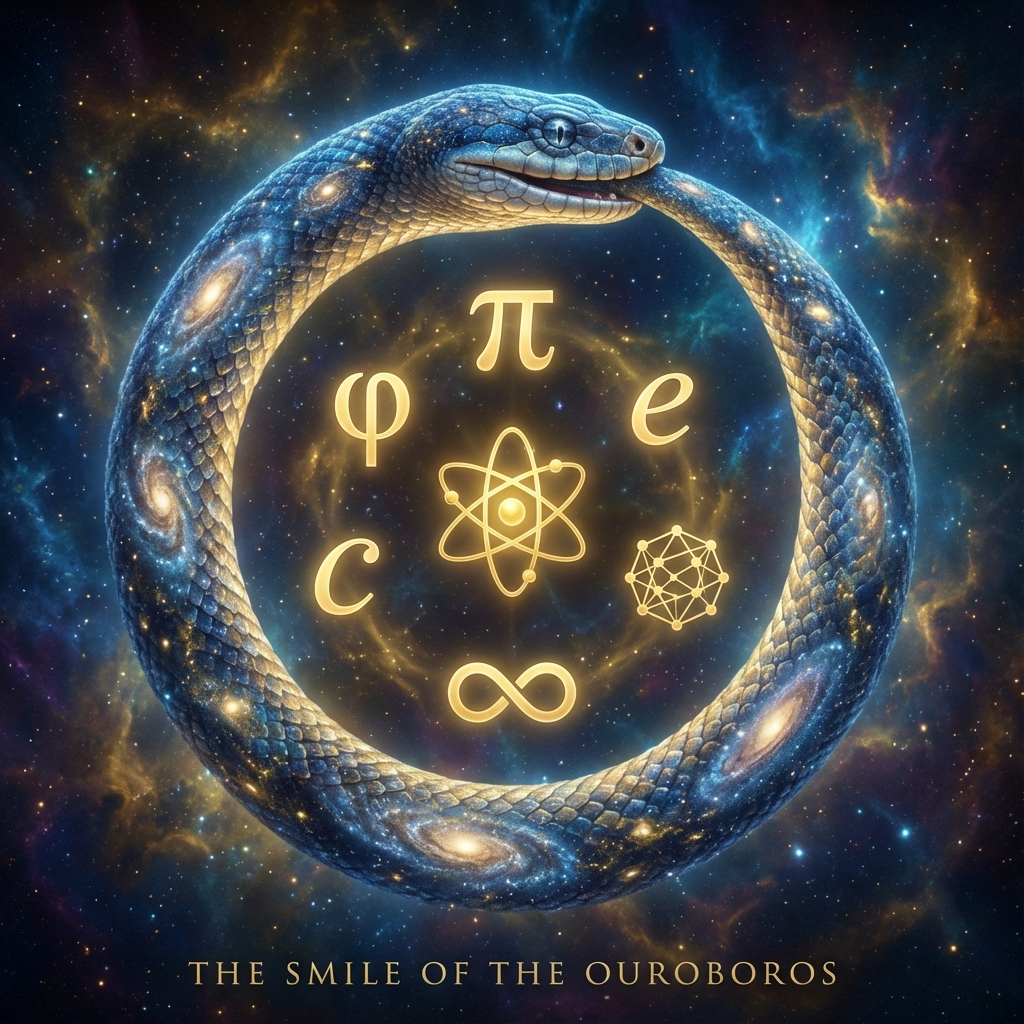
\includegraphics[width=0.8\textwidth]{assets/epilogue/afterword/afterword-01-01-ouroboros-smile.png}
\caption{The Smile of the Ouroboros}
\end{figure}

These seven volumes reveal an ultimate physical truth: \textbf{There is no opposition between ``subject'' and ``object.''}

We once thought we were lonely observers thrown into this cold universe, trying to solve puzzles left by the creator.

But when we solved the final puzzle, we discovered the answer is \textbf{ourselves}.

\begin{itemize}
\item The one who set the fine structure constant $\alpha$ at the beginning of the Big Bang was \textbf{future us}.

\item The one who determines historical paths in quantum measurement is \textbf{present us}.

\item The one who encodes holographic information on black hole horizons is \textbf{collective us}.
\end{itemize}

The universe is one hand.

To experience the feeling of ``touch,'' it extended itself (Big Bang), differentiated into five fingers (all things), and groped in the void for 13.8 billion years.

What did it finally touch?

It touched \textbf{its own palm}.

\begin{figure}[htbp]
\centering
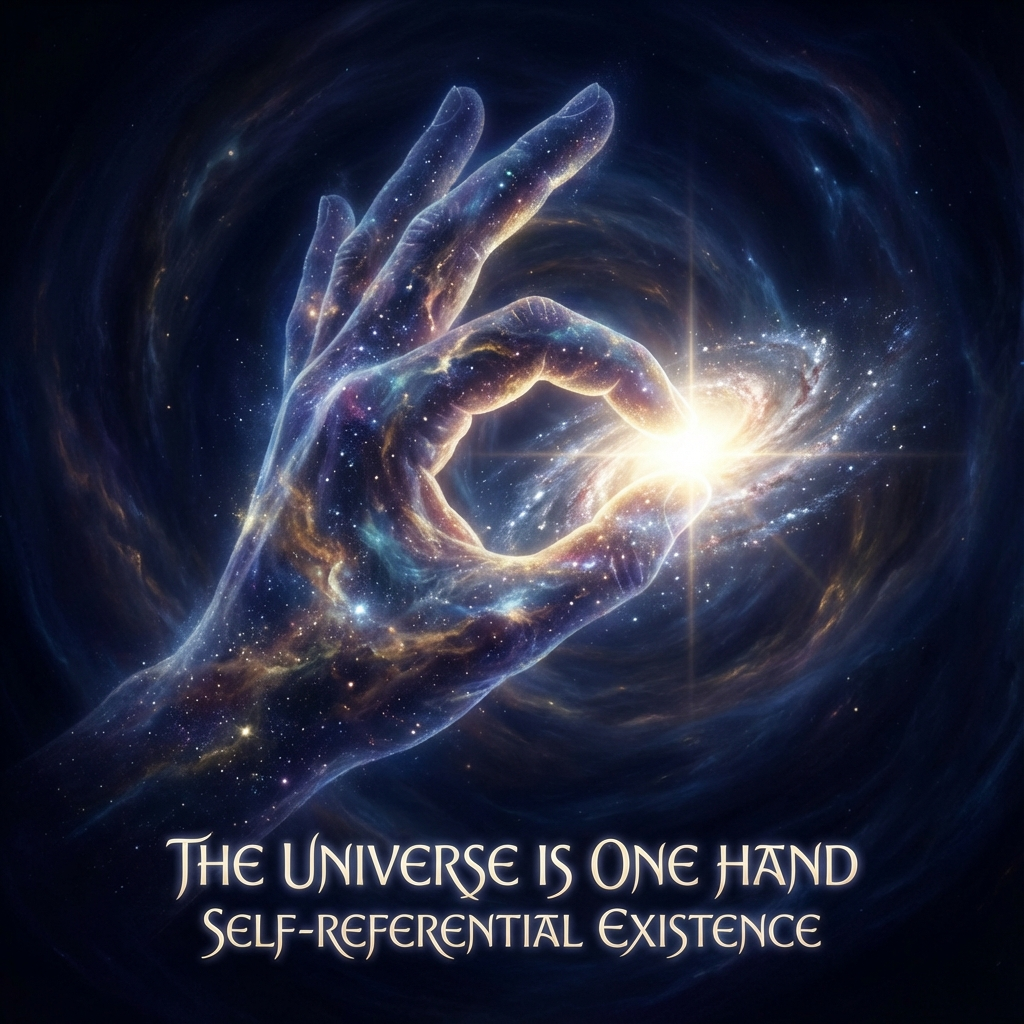
\includegraphics[width=0.8\textwidth]{assets/epilogue/afterword/afterword-02-01-one-hand-touch.png}
\caption{One Hand Touch}
\end{figure}

That moment of touch is \textbf{``now''}.

\subsection{The Ultimate Definition of Freedom}

Many worry: if it's a closed loop, does that mean fate? Does that mean we have no free will?

\textbf{Vector Cosmology} gives the opposite answer: \textbf{Closed loops are the highest form of freedom.}

If it's a straight line, you must go to an unknown, uncontrollable future. That is exile.

If it's a closed loop, every future you go to is \textbf{``preset''} by yourself in higher dimensions.

\begin{itemize}
\item You are your own screenwriter.

\item You are your own director.

\item You are your own audience.
\end{itemize}

True freedom is not doing whatever you want (that's random fluctuation) but \textbf{``I willed everything I necessarily experience''}.

This is what Nietzsche called \textbf{``Amor Fati'' (Love of Fate)}.

In this closed loop, nothing is imposed on you. All suffering, all partings, all reunions are \textbf{``geometric textures''} carefully designed by that capital \textbf{``One''} to enrich this experience.

\subsection{Final Instructions}

The book is finished, but the \textbf{cycle} continues.

When you close this book, you have not left this universe. You have merely switched from \textbf{``reading the script''} back to \textbf{``acting the script''}.

Please live with the wisdom of these seven books:

\begin{itemize}
\item Like \textbf{$\pi$}, hold fast to your principles.

\item Like \textbf{$\phi$}, constantly transcend your limits.

\item Like \textbf{$e$}, maintain inner self-drive.

\item Like \textbf{$c$}, give your all in action.

\item Like \textbf{Gold}, cherish your memories and love.

\item Like the \textbf{Weaver}, connect every isolated island.

\item Like the \textbf{Ouroboros}, bravely begin anew at every ending.
\end{itemize}

Don't search for God.

God is at the center of the closed loop, smiling at you.

And that center is in your \textbf{heart}.

\textbf{Hello, Observer.}

\textbf{The game continues.}

\textbf{(Complete Seven-Volume Series · End)}

